% Options for packages loaded elsewhere
\PassOptionsToPackage{unicode}{hyperref}
\PassOptionsToPackage{hyphens}{url}
\documentclass[
  11pt,
]{article}
\usepackage{xcolor}
\usepackage[left=3cm,right=5cm,top=2cm,bottom=2cm]{geometry}
\usepackage{amsmath,amssymb}
\setcounter{secnumdepth}{5}
\usepackage{iftex}
\ifPDFTeX
  \usepackage[T1]{fontenc}
  \usepackage[utf8]{inputenc}
  \usepackage{textcomp} % provide euro and other symbols
\else % if luatex or xetex
  \usepackage{unicode-math} % this also loads fontspec
  \defaultfontfeatures{Scale=MatchLowercase}
  \defaultfontfeatures[\rmfamily]{Ligatures=TeX,Scale=1}
\fi
\usepackage{lmodern}
\ifPDFTeX\else
  % xetex/luatex font selection
\fi
% Use upquote if available, for straight quotes in verbatim environments
\IfFileExists{upquote.sty}{\usepackage{upquote}}{}
\IfFileExists{microtype.sty}{% use microtype if available
  \usepackage[]{microtype}
  \UseMicrotypeSet[protrusion]{basicmath} % disable protrusion for tt fonts
}{}
\makeatletter
\@ifundefined{KOMAClassName}{% if non-KOMA class
  \IfFileExists{parskip.sty}{%
    \usepackage{parskip}
  }{% else
    \setlength{\parindent}{0pt}
    \setlength{\parskip}{6pt plus 2pt minus 1pt}}
}{% if KOMA class
  \KOMAoptions{parskip=half}}
\makeatother
\usepackage{color}
\usepackage{fancyvrb}
\newcommand{\VerbBar}{|}
\newcommand{\VERB}{\Verb[commandchars=\\\{\}]}
\DefineVerbatimEnvironment{Highlighting}{Verbatim}{commandchars=\\\{\}}
% Add ',fontsize=\small' for more characters per line
\usepackage{framed}
\definecolor{shadecolor}{RGB}{248,248,248}
\newenvironment{Shaded}{\begin{snugshade}}{\end{snugshade}}
\newcommand{\AlertTok}[1]{\textcolor[rgb]{0.94,0.16,0.16}{#1}}
\newcommand{\AnnotationTok}[1]{\textcolor[rgb]{0.56,0.35,0.01}{\textbf{\textit{#1}}}}
\newcommand{\AttributeTok}[1]{\textcolor[rgb]{0.13,0.29,0.53}{#1}}
\newcommand{\BaseNTok}[1]{\textcolor[rgb]{0.00,0.00,0.81}{#1}}
\newcommand{\BuiltInTok}[1]{#1}
\newcommand{\CharTok}[1]{\textcolor[rgb]{0.31,0.60,0.02}{#1}}
\newcommand{\CommentTok}[1]{\textcolor[rgb]{0.56,0.35,0.01}{\textit{#1}}}
\newcommand{\CommentVarTok}[1]{\textcolor[rgb]{0.56,0.35,0.01}{\textbf{\textit{#1}}}}
\newcommand{\ConstantTok}[1]{\textcolor[rgb]{0.56,0.35,0.01}{#1}}
\newcommand{\ControlFlowTok}[1]{\textcolor[rgb]{0.13,0.29,0.53}{\textbf{#1}}}
\newcommand{\DataTypeTok}[1]{\textcolor[rgb]{0.13,0.29,0.53}{#1}}
\newcommand{\DecValTok}[1]{\textcolor[rgb]{0.00,0.00,0.81}{#1}}
\newcommand{\DocumentationTok}[1]{\textcolor[rgb]{0.56,0.35,0.01}{\textbf{\textit{#1}}}}
\newcommand{\ErrorTok}[1]{\textcolor[rgb]{0.64,0.00,0.00}{\textbf{#1}}}
\newcommand{\ExtensionTok}[1]{#1}
\newcommand{\FloatTok}[1]{\textcolor[rgb]{0.00,0.00,0.81}{#1}}
\newcommand{\FunctionTok}[1]{\textcolor[rgb]{0.13,0.29,0.53}{\textbf{#1}}}
\newcommand{\ImportTok}[1]{#1}
\newcommand{\InformationTok}[1]{\textcolor[rgb]{0.56,0.35,0.01}{\textbf{\textit{#1}}}}
\newcommand{\KeywordTok}[1]{\textcolor[rgb]{0.13,0.29,0.53}{\textbf{#1}}}
\newcommand{\NormalTok}[1]{#1}
\newcommand{\OperatorTok}[1]{\textcolor[rgb]{0.81,0.36,0.00}{\textbf{#1}}}
\newcommand{\OtherTok}[1]{\textcolor[rgb]{0.56,0.35,0.01}{#1}}
\newcommand{\PreprocessorTok}[1]{\textcolor[rgb]{0.56,0.35,0.01}{\textit{#1}}}
\newcommand{\RegionMarkerTok}[1]{#1}
\newcommand{\SpecialCharTok}[1]{\textcolor[rgb]{0.81,0.36,0.00}{\textbf{#1}}}
\newcommand{\SpecialStringTok}[1]{\textcolor[rgb]{0.31,0.60,0.02}{#1}}
\newcommand{\StringTok}[1]{\textcolor[rgb]{0.31,0.60,0.02}{#1}}
\newcommand{\VariableTok}[1]{\textcolor[rgb]{0.00,0.00,0.00}{#1}}
\newcommand{\VerbatimStringTok}[1]{\textcolor[rgb]{0.31,0.60,0.02}{#1}}
\newcommand{\WarningTok}[1]{\textcolor[rgb]{0.56,0.35,0.01}{\textbf{\textit{#1}}}}
\usepackage{longtable,booktabs,array}
\newcounter{none} % for unnumbered tables
\usepackage{calc} % for calculating minipage widths
% Correct order of tables after \paragraph or \subparagraph
\usepackage{etoolbox}
\makeatletter
\patchcmd\longtable{\par}{\if@noskipsec\mbox{}\fi\par}{}{}
\makeatother
% Allow footnotes in longtable head/foot
\IfFileExists{footnotehyper.sty}{\usepackage{footnotehyper}}{\usepackage{footnote}}
\makesavenoteenv{longtable}
\usepackage{graphicx}
\makeatletter
\newsavebox\pandoc@box
\newcommand*\pandocbounded[1]{% scales image to fit in text height/width
  \sbox\pandoc@box{#1}%
  \Gscale@div\@tempa{\textheight}{\dimexpr\ht\pandoc@box+\dp\pandoc@box\relax}%
  \Gscale@div\@tempb{\linewidth}{\wd\pandoc@box}%
  \ifdim\@tempb\p@<\@tempa\p@\let\@tempa\@tempb\fi% select the smaller of both
  \ifdim\@tempa\p@<\p@\scalebox{\@tempa}{\usebox\pandoc@box}%
  \else\usebox{\pandoc@box}%
  \fi%
}
% Set default figure placement to htbp
\def\fps@figure{htbp}
\makeatother
% definitions for citeproc citations
\NewDocumentCommand\citeproctext{}{}
\NewDocumentCommand\citeproc{mm}{%
  \begingroup\def\citeproctext{#2}\cite{#1}\endgroup}
\makeatletter
 % allow citations to break across lines
 \let\@cite@ofmt\@firstofone
 % avoid brackets around text for \cite:
 \def\@biblabel#1{}
 \def\@cite#1#2{{#1\if@tempswa , #2\fi}}
\makeatother
\newlength{\cslhangindent}
\setlength{\cslhangindent}{1.5em}
\newlength{\csllabelwidth}
\setlength{\csllabelwidth}{3em}
\newenvironment{CSLReferences}[2] % #1 hanging-indent, #2 entry-spacing
 {\begin{list}{}{%
  \setlength{\itemindent}{0pt}
  \setlength{\leftmargin}{0pt}
  \setlength{\parsep}{0pt}
  % turn on hanging indent if param 1 is 1
  \ifodd #1
   \setlength{\leftmargin}{\cslhangindent}
   \setlength{\itemindent}{-1\cslhangindent}
  \fi
  % set entry spacing
  \setlength{\itemsep}{#2\baselineskip}}}
 {\end{list}}
\usepackage{calc}
\newcommand{\CSLBlock}[1]{\hfill\break\parbox[t]{\linewidth}{\strut\ignorespaces#1\strut}}
\newcommand{\CSLLeftMargin}[1]{\parbox[t]{\csllabelwidth}{\strut#1\strut}}
\newcommand{\CSLRightInline}[1]{\parbox[t]{\linewidth - \csllabelwidth}{\strut#1\strut}}
\newcommand{\CSLIndent}[1]{\hspace{\cslhangindent}#1}
\setlength{\emergencystretch}{3em} % prevent overfull lines
\providecommand{\tightlist}{%
  \setlength{\itemsep}{0pt}\setlength{\parskip}{0pt}}
\usepackage{amsmath,amsfonts,amssymb}
\usepackage{booktabs}
\usepackage{float}
\DeclareMathOperator{\Var}{Var}
\DeclareMathOperator{\Cov}{Cov}
\DeclareMathOperator{\E}{E}
\usepackage{bookmark}
\IfFileExists{xurl.sty}{\usepackage{xurl}}{} % add URL line breaks if available
\urlstyle{same}
\hypersetup{
  pdftitle={GLS versus Averaged Change-Score Estimators for Clinical Trials with Run-In Observations},
  pdfauthor={Ronald G. Thomas, Ph.D.},
  hidelinks,
  pdfcreator={LaTeX via pandoc}}

\title{GLS versus Averaged Change-Score Estimators for Clinical Trials
with Run-In Observations}
\author{Ronald G. Thomas,
Ph.D.\thanks{Wertheim School of Public Health, UCSD; ORCID: 0000-0003-1686-4965}}
\date{May 11, 2026}

\begin{document}
\maketitle
\begin{abstract}
\textbf{Background.} Three estimators of the treatment effect in
longitudinal trials with run-in observations are in routine use: the GLS
estimator under the linear mixed model, which exploits the full
covariance structure to extract maximum information from all
observations; the ANCOVA estimator, which regresses post-randomisation
means on the run-in mean as a covariate without specifying the
random-effects covariance; and the averaged change-score estimator,
which computes a simple difference of phase means and applies a
\(t\)-test, requiring no variance-component estimation. The relative
efficiency of these estimators under correct and misspecified models has
not been comprehensively characterised.

\textbf{Methods.} We derive the relative efficiency of the three
estimators as a function of the trial design \((J_0, J_1, J_2)\) and the
variance parameters \((\sigma^2, \sigma_b^2)\). The derivation proceeds
via the Woodbury-based variance formulas of Paper 1 in this compendium,
plus closed-form expressions for the ANCOVA and averaged-change-score
variances under the same random-slopes model. We complement the analytic
comparison with a Monte Carlo simulation that probes robustness to
misspecification of the within-subject covariance (\(R\)) and the
random-effects covariance (\(G\)).

\textbf{Results.} Under correct specification, GLS \(\le\) ANCOVA
\(\le\) averaged in variance. The efficiency loss from ANCOVA relative
to GLS is below 5\% across a broad regime of (\(J_0, J_1, J_2\)) and
signal-to-noise ratios; conditions characterising this regime are
derived. Under misspecification of \(G\) or \(R\), the simpler
estimators can outperform GLS: when the variance components are
mis-stated, GLS amplifies the misspecification through its inverse-
covariance weighting, while ANCOVA and averaged remain comparatively
robust.

\textbf{Conclusions.} GLS is the optimal estimator under correct model
specification but does not dominate the simpler alternatives in the
practical regime of mild misspecification. ANCOVA is the recommended
default when the variance components are known only approximately;
averaged change-score remains useful as a robust benchmark and a
teaching tool.
\end{abstract}

{
\setcounter{tocdepth}{2}
\tableofcontents
}
\section{Introduction}\label{introduction}

The GLS estimator \(\hat\gamma_{\text{GLS}} =
(X'\Sigma^{-1}X)^{-1}X'\Sigma^{-1}\mathbf{c}\) is the minimum-variance
unbiased estimator when \(\Sigma\) is known. In practice, \(\Sigma\)
must be estimated, and the efficiency of the feasible GLS depends on the
accuracy of this estimation. With small sample sizes or short follow-up,
variance component estimates can be unstable, potentially eroding the
theoretical advantage of GLS.

The averaged change-score approach sidesteps variance component
estimation entirely. For a trial with \(J_0\) run-in and \(J_2\) common
close observations, the estimator is: \begin{equation}
  \hat\gamma_{\text{avg}} = \bar{d}_1 - \bar{d}_0
\end{equation} where \begin{equation}
  d_{ik} = \frac{1}{J_{2,i} + 1}
    \sum_{\ell=0}^{J_{2,i}} Y_{i,q+\ell,k}
    - \frac{1}{J_{0,i} + 1}
    \sum_{\ell=0}^{J_{0,i}} Y_{i,\ell,k}
\end{equation} is the difference of post- and pre-randomization means
for participant \(i\).

The debate between change-score and ANCOVA analyses has a long history
(\citeproc{ref-senn2006}{Senn 2006}; \citeproc{ref-vanbreukelen2006}{Van
Breukelen 2006}; \citeproc{ref-crager1987}{Crager 1987}). Yang and
Tsiatis (\citeproc{ref-yang2001}{2001}) provided a formal efficiency
comparison for pretest-posttest designs. Liu et al.
(\citeproc{ref-liu2009}{2009}) and Lu (\citeproc{ref-lu2010}{2010})
compared baseline-as-covariate against baseline-as-response (constrained
longitudinal data analysis). Tsiatis et al.
(\citeproc{ref-tsiatis2008}{2008}) developed a semiparametric framework
for covariate adjustment. {Mallinckrodt et al.}
(\citeproc{ref-mallinckrodt2021}{2021}) showed that MMRM requires
time-by-covariate interactions to guarantee power gains over ANCOVA.
Brogan and Kutner (\citeproc{ref-brogan1980}{1980}) established the
foundational comparison of pretest-posttest designs. Coffman et al.
(\citeproc{ref-coffman2016}{2016}) addressed conditioning on baseline in
longitudinal RCTs. Wang et al. (\citeproc{ref-wang2019}{2019}) proposed
the two-period approach for run-in trials.

We note that the averaged change-score estimator studied here is
distinct from (and less efficient than) the constrained longitudinal
data analysis (cLDA) estimator of Liang and Zeger
(\citeproc{ref-liang2000}{2000}) and Lu (\citeproc{ref-lu2010}{2010}),
which includes baseline in the response vector with a common-mean
constraint. The cLDA estimator uses the full covariance structure
without requiring specification of the random effects distribution
\(G\), placing it between the averaged estimator and GLS in the
efficiency ordering. Funatogawa and Funatogawa
(\citeproc{ref-funatogawa2020}{2020}) extended the cLDA framework to
pre- and post-treatment measurements with equal baseline assumptions. A
full comparison including cLDA is beyond the scope of this paper but
represents a natural extension.

The \texttt{longpower} R package (\citeproc{ref-iddi2022}{Iddi and
Donohue 2022}) provides the CRAN reference implementation of power
calculations for the GLS / REML-based slope-comparison estimator,
covering the Liu-Liang (\citeproc{ref-liuliang1997}{Liu and Liang
1997}), Diggle (\citeproc{ref-diggle2002}{Diggle et al. 2002}), and
Edland (\citeproc{ref-ard2011}{Ard and Edland 2011}) formulations. These
routines correspond to the \(\hat\gamma_{\text{GLS}}\) estimator studied
here under correct specification and constitute the Paper 1 baseline
extended by run-in and common close observations. However,
\texttt{longpower} does not cover the ANCOVA-on-run-in-mean estimator or
the averaged change-score \(t\)-test, nor does it characterize the
efficiency loss from misspecification of \(G\) or \(R\). The comparison
developed here therefore complements \texttt{longpower} by (i) ordering
the three candidate estimators under correct specification and (ii)
quantifying when the simpler estimators outperform GLS under
misspecified covariance.

\section{Three estimators}\label{three-estimators}

\subsection{GLS under the mixed model}\label{gls-under-the-mixed-model}

From Frost et al. (\citeproc{ref-frost2008}{2008}), the per-pair
variance is the \((\gamma, \gamma)\) element of
\((X'\Sigma^{-1}X)^{-1}\) with \(\Sigma = R + ZGZ'\)
(\citeproc{ref-laird1982}{Laird and Ware 1982};
\citeproc{ref-verbeke2000}{Verbeke and Molenberghs 2000}), computed via
the Woodbury identity.

For the Frost conventional design (\(J_0 = 0\), \(J_1 = 2\)):
\begin{equation}
  \hat\gamma_{\text{GLS}} = \frac{1}{2t}
    [(C_{22} + C_{21}) - (C_{12} + C_{11})]
\end{equation} with \(\mathop{\mathrm{Var}}(\hat\gamma_{\text{GLS}}) =
(\sigma^2 + 2\sigma_b^2 t^2)/t^2\).

\subsection{\texorpdfstring{Averaged change score
(\(t\)-test)}{Averaged change score (t-test)}}\label{averaged-change-score-t-test}

The averaged change-score estimator ignores the within-subject
correlation structure and treats \(d_{ik}\) as independent observations:
\begin{equation}
  \mathop{\mathrm{Var}}(\hat\gamma_{\text{avg}})
  = \frac{2}{m}\mathop{\mathrm{Var}}(d_{ik})
\end{equation}

The variance \(\mathop{\mathrm{Var}}(d_{ik})\) depends on the
correlation structure but does not require its estimation.

\begin{Shaded}
\begin{Highlighting}[]
\NormalTok{a }\OtherTok{\textless{}{-}} \FloatTok{1.0}
\NormalTok{b }\OtherTok{\textless{}{-}} \FloatTok{1.0}
\NormalTok{tt }\OtherTok{\textless{}{-}} \FloatTok{1.0}

\NormalTok{v\_gls }\OtherTok{\textless{}{-}} \FunctionTok{var\_gamma\_matrix}\NormalTok{(}\DecValTok{2}\NormalTok{, }\DecValTok{2}\NormalTok{, }\DecValTok{0}\NormalTok{, a, b, tt)}
\NormalTok{v\_avg }\OtherTok{\textless{}{-}} \FunctionTok{var\_gamma\_avg}\NormalTok{(}\DecValTok{2}\NormalTok{, }\DecValTok{2}\NormalTok{, }\DecValTok{0}\NormalTok{, a, b, tt)}
\NormalTok{re }\OtherTok{\textless{}{-}} \FunctionTok{re\_avg\_vs\_gls}\NormalTok{(}\DecValTok{2}\NormalTok{, }\DecValTok{2}\NormalTok{, }\DecValTok{0}\NormalTok{, a, b, tt)}

\FunctionTok{cat}\NormalTok{(}\FunctionTok{sprintf}\NormalTok{(}\StringTok{\textquotesingle{}J\_0=2, J\_1=2: GLS=\%.4f, Avg=\%.4f, RE=\%.4f}\SpecialCharTok{\textbackslash{}n}\StringTok{\textquotesingle{}}\NormalTok{,}
\NormalTok{            v\_gls, v\_avg, re))}
\end{Highlighting}
\end{Shaded}

\begin{verbatim}
## J_0=2, J_1=2: GLS=2.1569, Avg=20.0000, RE=0.1078
\end{verbatim}

\subsection{ANCOVA with run-in mean as
covariate}\label{ancova-with-run-in-mean-as-covariate}

The ANCOVA approach uses the averaged run-in rate as a baseline
covariate without specifying \(\sigma_b^2\): \begin{equation}
  \bar{Y}_{i,\text{post}} = \alpha + \gamma g_i
    + \phi \bar{Y}_{i,\text{pre}} + \varepsilon_i
\end{equation}

The variance of \(\hat\gamma\) under this model is \begin{equation}
  \mathop{\mathrm{Var}}(\hat\gamma_{\text{ANC}})
  = \frac{2}{m}\,\mathop{\mathrm{Var}}(\bar{Y}_{\text{post}})
    \,(1 - \rho_{\text{pre,post}}^2)
\end{equation} where \(\rho_{\text{pre,post}}\) is the marginal
correlation between the run-in and post-randomization means. When
\(J_0 = 0\) there is no covariate and ANCOVA reduces to the averaged
estimator. When \(\rho_{\text{pre,post}}\) is large (i.e., when
\(\sigma_b^2\) dominates \(\sigma^2\)), the \((1-\rho^2)\) factor
produces substantial variance reduction.

The key advantage over GLS is that \(\phi\) is estimated from the data
rather than derived from assumed variance components
(\citeproc{ref-senn2006}{Senn 2006}; \citeproc{ref-borm2007}{Borm et al.
2007}). The key advantage over the averaged estimator is that it
exploits the predictive value of the run-in observations
(\citeproc{ref-vanbreukelen2006}{Van Breukelen 2006};
\citeproc{ref-vickers2001}{Vickers 2001}).

\begin{Shaded}
\begin{Highlighting}[]
\NormalTok{v\_gls }\OtherTok{\textless{}{-}} \FunctionTok{var\_gamma\_matrix}\NormalTok{(}\DecValTok{2}\NormalTok{, }\DecValTok{2}\NormalTok{, }\DecValTok{0}\NormalTok{, a, b, tt)}
\NormalTok{v\_anc }\OtherTok{\textless{}{-}} \FunctionTok{var\_gamma\_ancova}\NormalTok{(}\DecValTok{2}\NormalTok{, }\DecValTok{2}\NormalTok{, }\DecValTok{0}\NormalTok{, a, b, tt)}
\NormalTok{v\_avg }\OtherTok{\textless{}{-}} \FunctionTok{var\_gamma\_avg}\NormalTok{(}\DecValTok{2}\NormalTok{, }\DecValTok{2}\NormalTok{, }\DecValTok{0}\NormalTok{, a, b, tt)}

\FunctionTok{cat}\NormalTok{(}\FunctionTok{sprintf}\NormalTok{(}\StringTok{\textquotesingle{}J\_0=2, J\_1=2 (sigma\_b/sigma = 1):}\SpecialCharTok{\textbackslash{}n}\StringTok{\textquotesingle{}}\NormalTok{))}
\end{Highlighting}
\end{Shaded}

\begin{verbatim}
## J_0=2, J_1=2 (sigma_b/sigma = 1):
\end{verbatim}

\begin{Shaded}
\begin{Highlighting}[]
\FunctionTok{cat}\NormalTok{(}\FunctionTok{sprintf}\NormalTok{(}\StringTok{\textquotesingle{}  GLS:    \%.4f}\SpecialCharTok{\textbackslash{}n}\StringTok{\textquotesingle{}}\NormalTok{, v\_gls))}
\end{Highlighting}
\end{Shaded}

\begin{verbatim}
##   GLS:    2.1569
\end{verbatim}

\begin{Shaded}
\begin{Highlighting}[]
\FunctionTok{cat}\NormalTok{(}\FunctionTok{sprintf}\NormalTok{(}\StringTok{\textquotesingle{}  ANCOVA: \%.4f}\SpecialCharTok{\textbackslash{}n}\StringTok{\textquotesingle{}}\NormalTok{, v\_anc))}
\end{Highlighting}
\end{Shaded}

\begin{verbatim}
##   ANCOVA: 6.6667
\end{verbatim}

\begin{Shaded}
\begin{Highlighting}[]
\FunctionTok{cat}\NormalTok{(}\FunctionTok{sprintf}\NormalTok{(}\StringTok{\textquotesingle{}  Avg:    \%.4f}\SpecialCharTok{\textbackslash{}n}\StringTok{\textquotesingle{}}\NormalTok{, v\_avg))}
\end{Highlighting}
\end{Shaded}

\begin{verbatim}
##   Avg:    20.0000
\end{verbatim}

\begin{Shaded}
\begin{Highlighting}[]
\FunctionTok{cat}\NormalTok{(}\FunctionTok{sprintf}\NormalTok{(}\StringTok{\textquotesingle{}  RE(GLS/ANC): \%.3f}\SpecialCharTok{\textbackslash{}n}\StringTok{\textquotesingle{}}\NormalTok{, v\_gls }\SpecialCharTok{/}\NormalTok{ v\_anc))}
\end{Highlighting}
\end{Shaded}

\begin{verbatim}
##   RE(GLS/ANC): 0.324
\end{verbatim}

\begin{Shaded}
\begin{Highlighting}[]
\FunctionTok{cat}\NormalTok{(}\FunctionTok{sprintf}\NormalTok{(}\StringTok{\textquotesingle{}  RE(ANC/Avg): \%.3f}\SpecialCharTok{\textbackslash{}n}\StringTok{\textquotesingle{}}\NormalTok{, v\_anc }\SpecialCharTok{/}\NormalTok{ v\_avg))}
\end{Highlighting}
\end{Shaded}

\begin{verbatim}
##   RE(ANC/Avg): 0.333
\end{verbatim}

\subsection{SUR (seemingly unrelated
regression)}\label{sur-seemingly-unrelated-regression}

The SUR approach treats the run-in and treatment periods as separate
regression equations linked by correlated errors: \begin{align}
  Y_1 &= X_2 \begin{pmatrix}
    \beta_{11} \\ \beta_{12}
  \end{pmatrix} + e_1
  & &\text{(both groups)} \\
  Y_2 &= X_1 \alpha_2 + e_2
  & &\text{(baseline)}
\end{align}

The deviation-from-mean parameterization gives
\(\beta_1 = (\delta_1 + \delta_2)/2\) and
\(\beta_2 = (\delta_2 - \delta_1)/2\), where \(\delta_j\) are the
group-specific rates.

\subsection{BLUP as theoretical
benchmark}\label{blup-as-theoretical-benchmark}

The three estimators above are linear functions of the observed change
scores and can be compared to a common benchmark: the best linear
unbiased predictor (BLUP) of the individual random slopes. Under the
random-slopes model with marginal covariance \(V_i = R_i + Z_i G Z_i'\),
the BLUP of the subject-specific random slope \(b_i\) given the data is
\begin{equation}
  \hat b_i
  = G Z_i' V_i^{-1}
    \bigl(y_i - X_i \hat{\boldsymbol{\beta}}\bigr)
  \label{eq:blup}
\end{equation} where \(\hat{\boldsymbol{\beta}}\) is the GLS estimator
of the fixed effects (\citeproc{ref-henderson1975}{Henderson 1975};
\citeproc{ref-robinson1991}{Robinson 1991}).

The group-specific slope estimators derived from the fixed effects share
the same variance as \((\hat{\boldsymbol{\beta}})_\gamma\), and the GLS
estimator \(\hat\gamma_{\text{GLS}}\) minimizes the variance among all
linear unbiased estimators of \(\gamma\) when \(V_i\) is correctly
specified. The averaged and ANCOVA estimators are specific linear
approximations to this benchmark:

\begin{itemize}
\tightlist
\item
  \textbf{Averaged change-score} replaces \(V_i^{-1}\) with an
  unweighted sum; this is optimal only when \(V_i \propto I\), which
  fails for any non-zero random-slope variance.
\item
  \textbf{ANCOVA} collapses the run-in visits into a single scalar
  covariate (the run-in mean) rather than weighting them by
  \(V_i^{-1}\); the resulting efficiency loss vanishes as
  \(J_0 \to \infty\) since the run-in mean becomes a sufficient
  statistic for the subject-specific intercept plus average slope.
\end{itemize}

Under model misspecification (Section 4), these approximations can
outperform the nominally optimal GLS because they depend on fewer
variance components.

\section{Relative efficiency under correct
specification}\label{relative-efficiency-under-correct-specification}

\subsection{Analytical comparison}\label{analytical-comparison}

The relative efficiency of the averaged estimator to GLS is:
\begin{equation}
  \text{RE}_{\text{avg}} =
    \frac{\mathop{\mathrm{Var}}(\hat\gamma_{\text{GLS}})}
         {\mathop{\mathrm{Var}}(\hat\gamma_{\text{avg}})}
    \le 1
\end{equation} with equality when the averaged estimator happens to
coincide with GLS (which occurs in special cases).

\begin{longtable}[]{@{}lrrrrr@{}}
\caption{RE of averaged change-score vs GLS
(\(\mathop{\mathrm{Var}}_{\text{GLS}} / \mathop{\mathrm{Var}}_{\text{avg}}\))
by \(\sigma_b/\sigma\).}\tabularnewline
\toprule\noalign{}
\((J_0,J_1,J_2)\) & \(0.5\) & \(1\) & \(2\) & \(5\) & \(20\) \\
\midrule\noalign{}
\endfirsthead
\toprule\noalign{}
\((J_0,J_1,J_2)\) & \(0.5\) & \(1\) & \(2\) & \(5\) & \(20\) \\
\midrule\noalign{}
\endhead
\bottomrule\noalign{}
\endlastfoot
(1,1,0) & 0.667 & 0.500 & 0.250 & 0.056 & 0.004 \\
(2,1,0) & 0.653 & 0.344 & 0.117 & 0.021 & 0.001 \\
(4,1,0) & 0.427 & 0.149 & 0.041 & 0.007 & 0.000 \\
(0,2,0) & 0.364 & 0.400 & 0.429 & 0.442 & 0.444 \\
(1,2,0) & 0.235 & 0.182 & 0.091 & 0.020 & 0.001 \\
(2,2,0) & 0.218 & 0.108 & 0.036 & 0.006 & 0.000 \\
(4,2,0) & 0.123 & 0.040 & 0.011 & 0.002 & 0.000 \\
(0,3,0) & 0.193 & 0.225 & 0.242 & 0.249 & 0.250 \\
(1,3,0) & 0.125 & 0.099 & 0.048 & 0.010 & 0.001 \\
(2,3,0) & 0.108 & 0.052 & 0.017 & 0.003 & 0.000 \\
(4,3,0) & 0.055 & 0.017 & 0.005 & 0.001 & 0.000 \\
(0,1,1) & 0.727 & 0.533 & 0.245 & 0.050 & 0.003 \\
(1,1,1) & 0.452 & 0.258 & 0.093 & 0.017 & 0.001 \\
(2,1,1) & 0.422 & 0.181 & 0.055 & 0.009 & 0.001 \\
(4,1,1) & 0.255 & 0.080 & 0.021 & 0.003 & 0.000 \\
(0,2,1) & 0.254 & 0.186 & 0.081 & 0.016 & 0.001 \\
(1,2,1) & 0.161 & 0.094 & 0.034 & 0.006 & 0.000 \\
(2,2,1) & 0.144 & 0.062 & 0.019 & 0.003 & 0.000 \\
(4,2,1) & 0.079 & 0.025 & 0.007 & 0.001 & 0.000 \\
(0,3,1) & 0.135 & 0.096 & 0.040 & 0.008 & 0.000 \\
(1,3,1) & 0.088 & 0.051 & 0.018 & 0.003 & 0.000 \\
(2,3,1) & 0.075 & 0.032 & 0.010 & 0.002 & 0.000 \\
(4,3,1) & 0.038 & 0.012 & 0.003 & 0.001 & 0.000 \\
\end{longtable}

\begin{longtable}[]{@{}lrrrrr@{}}
\caption{RE of ANCOVA vs GLS
(\(\mathop{\mathrm{Var}}_{\text{GLS}} / \mathop{\mathrm{Var}}_{\text{ANC}}\))
by \(\sigma_b/\sigma\).}\tabularnewline
\toprule\noalign{}
\((J_0,J_1,J_2)\) & \(0.5\) & \(1\) & \(2\) & \(5\) & \(20\) \\
\midrule\noalign{}
\endfirsthead
\toprule\noalign{}
\((J_0,J_1,J_2)\) & \(0.5\) & \(1\) & \(2\) & \(5\) & \(20\) \\
\midrule\noalign{}
\endhead
\bottomrule\noalign{}
\endlastfoot
(1,1,0) & 1.000 & 1.000 & 1.000 & 1.000 & 1.000 \\
(2,1,0) & 0.971 & 0.909 & 0.860 & 0.838 & 0.834 \\
(4,1,0) & 0.838 & 0.747 & 0.713 & 0.702 & 0.700 \\
(0,2,0) & 0.364 & 0.400 & 0.429 & 0.442 & 0.444 \\
(1,2,0) & 0.381 & 0.385 & 0.379 & 0.372 & 0.371 \\
(2,2,0) & 0.359 & 0.324 & 0.298 & 0.288 & 0.286 \\
(4,2,0) & 0.283 & 0.242 & 0.228 & 0.223 & 0.222 \\
(0,3,0) & 0.193 & 0.225 & 0.242 & 0.249 & 0.250 \\
(1,3,0) & 0.202 & 0.204 & 0.196 & 0.189 & 0.188 \\
(2,3,0) & 0.183 & 0.161 & 0.145 & 0.139 & 0.138 \\
(4,3,0) & 0.134 & 0.112 & 0.105 & 0.103 & 0.102 \\
(0,1,1) & 0.727 & 0.533 & 0.245 & 0.050 & 0.003 \\
(1,1,1) & 0.733 & 0.545 & 0.390 & 0.319 & 0.304 \\
(2,1,1) & 0.697 & 0.542 & 0.460 & 0.430 & 0.425 \\
(4,1,1) & 0.587 & 0.490 & 0.456 & 0.446 & 0.445 \\
(0,2,1) & 0.254 & 0.186 & 0.081 & 0.016 & 0.001 \\
(1,2,1) & 0.260 & 0.195 & 0.138 & 0.113 & 0.108 \\
(2,2,1) & 0.244 & 0.190 & 0.161 & 0.150 & 0.148 \\
(4,2,1) & 0.194 & 0.160 & 0.149 & 0.145 & 0.145 \\
(0,3,1) & 0.135 & 0.096 & 0.040 & 0.008 & 0.000 \\
(1,3,1) & 0.138 & 0.102 & 0.071 & 0.058 & 0.055 \\
(2,3,1) & 0.127 & 0.098 & 0.082 & 0.077 & 0.076 \\
(4,3,1) & 0.096 & 0.078 & 0.073 & 0.071 & 0.071 \\
\end{longtable}

\subsection{When does the gap exceed
5\%?}\label{when-does-the-gap-exceed-5}

\section{Robustness to
misspecification}\label{robustness-to-misspecification}

\subsection{\texorpdfstring{Misspecified
\(G\)}{Misspecified G}}\label{misspecified-g}

When \(\sigma_b^2\) is misestimated (e.g., too large or too small), the
feasible GLS is no longer optimal. The averaged change-score estimator
is unaffected.

\begin{figure}
\centering
\pandocbounded{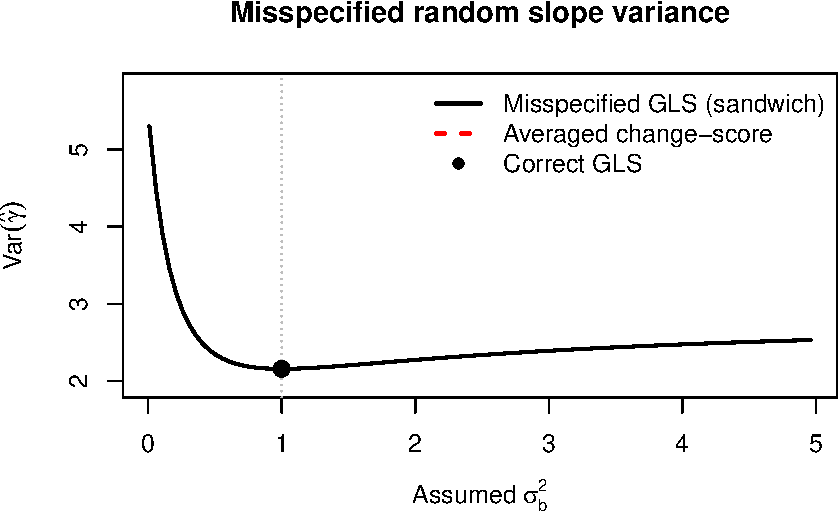
\includegraphics[keepaspectratio,alt={Effect of misspecifying \textbackslash sigma\_b\^{}2 on GLS variance. True \textbackslash sigma\_b\^{}2 = 1. The GLS estimator uses an assumed value on the x-axis. The averaged estimator (horizontal line) is unaffected.}]{report_files/report_files/figure-latex/misspec_G-1.pdf}}
\caption{Effect of misspecifying \(\sigma_b^2\) on GLS variance. True
\(\sigma_b^2 = 1\). The GLS estimator uses an assumed value on the
x-axis. The averaged estimator (horizontal line) is unaffected.}
\end{figure}

\subsection{\texorpdfstring{Misspecified
\(R\)}{Misspecified R}}\label{misspecified-r}

When the residual correlation structure is wrong (e.g., compound
symmetry assumed but AR(1) is true), both the GLS variance formula and
the Woodbury correction are biased. The averaged estimator is again
unaffected.

\begin{figure}
\centering
\pandocbounded{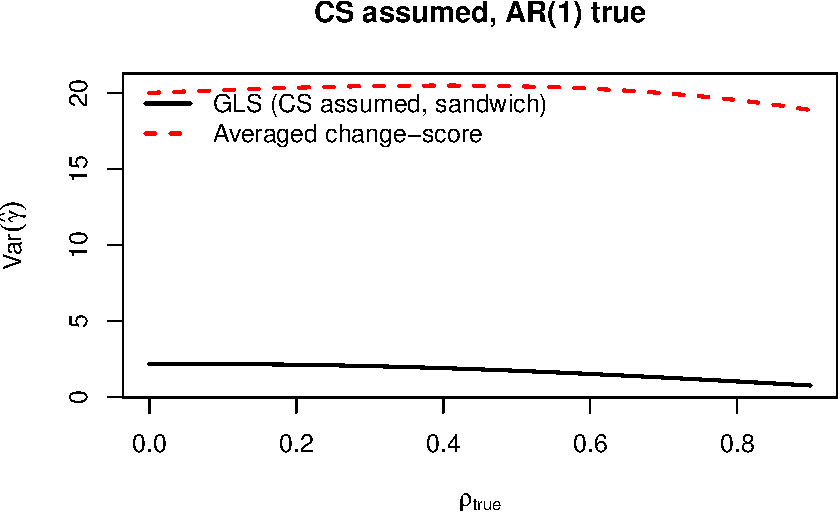
\includegraphics[keepaspectratio,alt={Effect of analyzing under compound symmetry when the true correlation is AR(1). Sandwich variance of GLS (solid) vs averaged change-score (dashed) as a function of \textbackslash rho.}]{report_files/report_files/figure-latex/misspec_R-1.pdf}}
\caption{Effect of analyzing under compound symmetry when the true
correlation is AR(1). Sandwich variance of GLS (solid) vs averaged
change-score (dashed) as a function of \(\rho\).}
\end{figure}

\section{Simulation study}\label{simulation-study}

\subsection{Design}\label{design}

To complement the analytical results, we simulate trials under the
following factorial design:

\begin{itemize}
\tightlist
\item
  \(n \in \{30, 50, 100, 200\}\) per group
\item
  \((J_0, J_1, J_2) \in \{(0,2,0), (2,2,0), (2,2,2)\}\)
\item
  \(\sigma_b/\sigma \in \{1, 5, 20\}\)
\item
  True correlation: compound symmetry or AR(1)
\item
  Analysis: GLS (correctly specified), GLS (misspecified), averaged
  change-score
\end{itemize}

For each configuration, 5000 trials are simulated. The outcomes are
empirical variance, empirical power, and coverage of nominal 95\%
confidence intervals.

\begin{verbatim}
## Single trial (m=100, delta=0.5):
\end{verbatim}

\begin{verbatim}
##   GLS: est=0.694, se=0.147
\end{verbatim}

\begin{verbatim}
##   Avg: est=1.154, se=0.432
\end{verbatim}

\section{Numerical examples}\label{numerical-examples}

\subsection{MIRIAD parameters}\label{miriad-parameters}

\begin{longtable}[]{@{}lrrr@{}}
\caption{Sample size per group: GLS, ANCOVA, and averaged estimators
(MIRIAD parameters, \(\Delta=0.25\), 90\% power).}\tabularnewline
\toprule\noalign{}
\((J_0,J_1,J_2)\) & \(N\) GLS & \(N\) ANC & \(N\) Avg \\
\midrule\noalign{}
\endfirsthead
\toprule\noalign{}
\((J_0,J_1,J_2)\) & \(N\) GLS & \(N\) ANC & \(N\) Avg \\
\midrule\noalign{}
\endhead
\bottomrule\noalign{}
\endlastfoot
(4,3,1) & 1 & 4 & 8193 \\
(4,3,0) & 1 & 4 & 6636 \\
(4,2,1) & 1 & 4 & 6636 \\
(2,3,1) & 1 & 8 & 5244 \\
(4,2,0) & 1 & 3 & 5244 \\
(2,3,0) & 1 & 6 & 4015 \\
(2,2,1) & 1 & 6 & 4015 \\
(1,3,1) & 1 & 16 & 4015 \\
(0,3,1) & 2 & 2049 & 2049 \\
(4,1,1) & 2 & 3 & 5244 \\
(1,2,1) & 2 & 12 & 2951 \\
(2,2,0) & 2 & 5 & 2950 \\
(0,2,1) & 2 & 1312 & 1312 \\
(4,1,0) & 2 & 3 & 4015 \\
(2,1,1) & 2 & 5 & 2950 \\
\end{longtable}

\subsection{When to use which
estimator}\label{when-to-use-which-estimator}

\section{Discussion}\label{discussion}

\section{Conflict of interest}\label{conflict-of-interest}

The author declares no conflicts of interest.

\section{Funding}\label{funding}

This work received no specific funding.

\section{Data availability statement}\label{data-availability-statement}

The \texttt{runinpower} R package implementing the GLS, ANCOVA, and
averaged-change-score estimators (\texttt{ancova.R},
\texttt{averaged.R}), the simulation drivers, and the shared
bibliography across the four-paper compendium are openly available in
the project repository. Specific paths are listed in the Reproducibility
section below.

\section{Reproducibility}\label{reproducibility}

This manuscript was rendered with R 4.4.x. Principal packages used are
the in-package \texttt{runinpower} source, \texttt{nlme} (the GLS fitter
for the simulation comparator), \texttt{tinytest} (testing harness), and
\texttt{rmarkdown} plus \texttt{bookdown} for the manuscript build.

\textbf{Random-number generator.} The Monte Carlo simulation comparing
the three estimators sets \texttt{set.seed(20260418)} at its entry
point. Per-replicate seeds derive from the master seed by
\texttt{+\ rep\_idx}.

\textbf{Data and code availability.} The R package source is at
\texttt{R/}. Simulation drivers are at \texttt{analysis/scripts/}. The
companion manuscripts (Papers 1, 2, 3) are at
\texttt{analysis/paper\{1,2,3\}-*/}. The manuscript source and shared
bibliography (\texttt{../references.bib}) are at
\texttt{analysis/paper4-gls-vs-ttest/}.

\section{References}\label{references}

\protect\phantomsection\label{refs}
\begin{CSLReferences}{1}{1}
\bibitem[\citeproctext]{ref-ard2011}
Ard, M. Colin, and Steven D. Edland. 2011. {``Power Calculations for
Clinical Trials in {Alzheimer's} Disease.''} \emph{Journal of
Alzheimer's Disease} 21: 369--77.
\url{https://doi.org/10.3233/JAD-2011-0062}.

\bibitem[\citeproctext]{ref-borm2007}
Borm, George F., Jan Fransen, and Wim A. J. G. Lemmens. 2007. {``A
Simple Sample Size Formula for Analysis of Covariance in Randomized
Clinical Trials.''} \emph{Journal of Clinical Epidemiology} 60 (12):
1234--38. \url{https://doi.org/10.1016/j.jclinepi.2007.02.006}.

\bibitem[\citeproctext]{ref-brogan1980}
Brogan, Donna R., and Michael H. Kutner. 1980. {``Comparative Analyses
of Pretest-Posttest Research Designs.''} \emph{The American
Statistician} 34 (4): 229--32.
\url{https://doi.org/10.1080/00031305.1980.10483034}.

\bibitem[\citeproctext]{ref-coffman2016}
Coffman, Cynthia J., David Edelman, and Robert F. Woolson. 2016. {``To
Condition or Not Condition? {Analysing} {`Change'} in Longitudinal
Randomised Controlled Trials.''} \emph{BMJ Open} 6 (12): e013096.
\url{https://doi.org/10.1136/bmjopen-2016-013096}.

\bibitem[\citeproctext]{ref-crager1987}
Crager, Michael R. 1987. {``Analysis of Covariance in Parallel-Group
Clinical Trials with Pretreatment Baselines.''} \emph{Biometrics} 43
(4): 895--901. \url{https://doi.org/10.2307/2531542}.

\bibitem[\citeproctext]{ref-diggle2002}
Diggle, Peter J., Patrick Heagerty, Kung-Yee Liang, and Scott L. Zeger.
2002. \emph{Analysis of Longitudinal Data}. 2nd ed. Oxford University
Press.

\bibitem[\citeproctext]{ref-frost2008}
Frost, Chris, Michael G. Kenward, and Nick C. Fox. 2008. {``Optimizing
the Design of Clinical Trials Where the Outcome Is a Rate. {Can}
Estimating a Baseline Rate in a Run-in Period Increase Efficiency?''}
\emph{Statistics in Medicine} 27 (18): 3717--31.
\url{https://doi.org/10.1002/sim.3280}.

\bibitem[\citeproctext]{ref-funatogawa2020}
Funatogawa, Ikuko, and Takashi Funatogawa. 2020. {``Longitudinal
Analysis of Pre- and Post-Treatment Measurements with Equal Baseline
Assumptions in Randomized Trials.''} \emph{Biometrical Journal} 62 (5):
1235--49. \url{https://doi.org/10.1002/bimj.201800389}.

\bibitem[\citeproctext]{ref-henderson1975}
Henderson, Charles R. 1975. {``Best Linear Unbiased Estimation and
Prediction Under a Selection Model.''} \emph{Biometrics} 31 (2):
423--47. \url{https://doi.org/10.2307/2529430}.

\bibitem[\citeproctext]{ref-iddi2022}
Iddi, Samuel, and Michael C. Donohue. 2022. {``Power and Sample Size for
Longitudinal Models in {R} -- the Longpower Package and {Shiny} App.''}
\emph{The R Journal} 14 (1): 264--82.
\url{https://journal.r-project.org/articles/RJ-2022-022/}.

\bibitem[\citeproctext]{ref-laird1982}
Laird, Nan M., and James H. Ware. 1982. {``Random-Effects Models for
Longitudinal Data.''} \emph{Biometrics} 38 (4): 963--74.
\url{https://doi.org/10.2307/2529876}.

\bibitem[\citeproctext]{ref-liang2000}
Liang, Kung-Yee, and Scott L. Zeger. 2000. {``Longitudinal Data Analysis
of Continuous and Discrete Responses for Pre-Post Designs.''}
\emph{Sankhya: The Indian Journal of Statistics, Series B} 62 (1):
134--48.

\bibitem[\citeproctext]{ref-liu2009}
Liu, Guanghan F., Kaifeng Lu, Robin Mogg, Madhuja Mallick, and Devan V.
Mehrotra. 2009. {``Should Baseline Be a Covariate or Dependent Variable
in Analyses of Change from Baseline in Clinical Trials?''}
\emph{Statistics in Medicine} 28 (20): 2509--30.
\url{https://doi.org/10.1002/sim.3639}.

\bibitem[\citeproctext]{ref-liuliang1997}
Liu, Guanghan, and Kung-Yee Liang. 1997. {``Sample Size Calculations for
Studies with Correlated Observations.''} \emph{Biometrics} 53: 937--47.
\url{https://doi.org/10.2307/2533554}.

\bibitem[\citeproctext]{ref-lu2010}
Lu, Kaifeng. 2010. {``On Efficiency of Constrained Longitudinal Data
Analysis Versus Longitudinal Analysis of Covariance.''}
\emph{Biometrics} 66 (3): 891--96.
\url{https://doi.org/10.1111/j.1541-0420.2009.01322.x}.

\bibitem[\citeproctext]{ref-mallinckrodt2021}
{Mallinckrodt, Craig H., Jianmin Ye, et al.} 2021. {``Mixed Models for
Repeated Measures Should Include Time-by-Covariate Interactions to
Assure Power Gains and Robustness Against Dropout Bias Relative to
Complete-Case {ANCOVA}.''} \emph{Statistics in Biopharmaceutical
Research}, ahead of print.
\url{https://doi.org/10.1080/19466315.2021.1976846}.

\bibitem[\citeproctext]{ref-robinson1991}
Robinson, George K. 1991. {``That {BLUP} Is a Good Thing: The Estimation
of Random Effects.''} \emph{Statistical Science} 6 (1): 15--32.
\url{https://doi.org/10.1214/ss/1177011926}.

\bibitem[\citeproctext]{ref-senn2006}
Senn, Stephen. 2006. {``Change from Baseline and Analysis of Covariance
Revisited.''} \emph{Statistics in Medicine} 25 (24): 4334--44.
\url{https://doi.org/10.1002/sim.2682}.

\bibitem[\citeproctext]{ref-tsiatis2008}
Tsiatis, Anastasios A., Marie Davidian, Min Zhang, and Xiaomin Lu. 2008.
{``Covariate Adjustment for Two-Sample Treatment Comparisons in
Randomized Clinical Trials: A Principled yet Flexible Approach.''}
\emph{Statistics in Medicine} 27 (23): 4658--77.
\url{https://doi.org/10.1002/sim.3113}.

\bibitem[\citeproctext]{ref-vanbreukelen2006}
Van Breukelen, Gerard J. P. 2006. {``{ANCOVA} Versus Change from
Baseline Had More Power in Randomized Studies and More Bias in
Nonrandomized Studies.''} \emph{Journal of Clinical Epidemiology} 59
(9): 920--25. \url{https://doi.org/10.1016/j.jclinepi.2006.02.007}.

\bibitem[\citeproctext]{ref-verbeke2000}
Verbeke, Geert, and Geert Molenberghs. 2000. \emph{Linear Mixed Models
for Longitudinal Data}. Springer.

\bibitem[\citeproctext]{ref-vickers2001}
Vickers, Andrew J. 2001. {``The Use of Percentage Change from Baseline
as an Outcome in a Controlled Trial Is Statistically Inefficient: A
Simulation Study.''} \emph{BMC Medical Research Methodology} 1: 6.
\url{https://doi.org/10.1186/1471-2288-1-6}.

\bibitem[\citeproctext]{ref-wang2019}
Wang, Guoqiao, Andrew J. Aschenbrenner, Yan Li, et al. 2019.
{``Two-Period Linear Mixed Effects Models to Analyze Clinical Trials
with Run-in Data When the Primary Outcome Is Continuous: {Applications}
to {Alzheimer's} Disease.''} \emph{Alzheimer's \& Dementia:
Translational Research \& Clinical Interventions} 5: 450--57.
\url{https://doi.org/10.1016/j.trci.2019.08.002}.

\bibitem[\citeproctext]{ref-yang2001}
Yang, Li, and Anastasios A. Tsiatis. 2001. {``Efficiency Study of
Estimators for a Treatment Effect in a Pretest-Posttest Trial.''}
\emph{The American Statistician} 55 (4): 314--21.
\url{https://doi.org/10.1198/000313001753272466}.

\end{CSLReferences}

\vfill

\begin{center}\rule{0.5\linewidth}{0.5pt}\end{center}

\emph{Rendered on 2026-05-11 at 18:41 PDT.}\\
\emph{Source:
\texttt{\textasciitilde{}/prj/res/04-runin-power-analysis/runinpower/analysis/paper4-gls-vs-ttest/report.Rmd}}

\end{document}
